%!TEX root=../thesis.tex
\chapter{Experiments}\label{chp:experiments}

% + behaviour with changing bandwidth -> analytical vs. CR results (see paper)
% + deep code restructure from original tool to v2.0
% + test to check that the new version of the tool gives correct results
%   comparing them with the ones obtained with the old tool on the same input
% + performance enhencment in matrix creation (see Bernardo's emails) [rememer to put reference
%   in the prosit overview chapter]

The version of PROSIT described in this thesis brings several improvements in the project format, especially in the core classes that holds the functions and the parameters connected to a task. Big changes in the code structure imply a complete revision of the results, even though they have been deeply checked in the "old" version of the tool.\\
This decision was not painless at all but is was necessary: PROSIT have been mainly developed and used in some papers\footnote{An example of paper which involved PROSIT to compute some results is \cite{probGuarantees}.} and the code structure was not an absolute priority at that moment. Then it gained interest, due to its capability to provide a good abstraction for many of the foundamental concepts during the design of real-time systems. For this reason the project has been modified following a new approach.\\
The changes in the structure of the code made necessary to check that the results provided by this "new" version does not contain or introduce any error. This phase of testing has been done by running multiple tasks with different parameters on both versions and then checking the correctness of the results. None inconsistency in the results was found while comparing the two versions.\\
The process of testing and comparison described above was done in an automated way using some scripts written in bash.

\section{Cyclic Reduction accuracy} \label{craccuracy}
In order to compare the accuracy between the analytical and the Cyclic Reduction algorithms, a task with the same parameters (except for the bandwith) is considered. The budget \( Q_{i}^{s} \) is changed to make the bandwith value in the range [35\% - 60\%]. The results with a granularity of 50\,\( \mu{s} \) are visible in the table below.
\begin{table}[H]
\label{comparison}
\begin{center}
\begin{tabular}{| l | l | l | l | l | l |}
  \hline
  Bandwith & 35\% & 40\% & 45\% & 50\% & 60\% \\ \hline
  Analitic bound & 0.602 & 0.809 & 0.906 & 0.956 & 0.991 \\
  CR algorithm & 0.773 & 0.878 & 0.929 & 0.965 & 0.992 \\ \hline
\end{tabular}
\caption[]{Probabilities for different values of bandwith\footnotemark[2].}
\end{center} 
\end{table}

\footnotetext[2]{The results were evaluated on an Intel Core i7-3537U CPU @ 2.00GHz with 8GB of RAM.}

The gap between the results of the two different algorithms is significant in the first two columns, but it constantly decreases as the bandwith increases. A bandwith value lower than 40\% gives a probability to meet the deadline smaller than the 80\%, which is not sufficient for most of the real-time applications\footnote[3]{The QoS with this probability value would not allow the user to enjoy any real-time service.}.\\
This means that the CR works pretty well only in \emph{heavy-traffic} conditions, namely a situation in which the system is heavily used and stressed by many tasks. Luckily it is a standard situation for most of soft real-time systems.  

\section{Performance enhancement in matrix creation} \label{matrixperformance}
As described in Section \ref{matrixcreation}, the efficiency of the matrix creation has been highly improved. The table below shows a benchmark for an example matrix.
\begin{table}[H]
\label{benchmark}
\begin{center}
\begin{tabular}{| l | l |}
  \hline
  Matrix size & 442 \\ \hline
  Elapsed time "old" & 121238\( \,\mu{s} \) \\ \hline
  Elapsed time "new" & 71413\( \,\mu{s} \) \\ \hline
\end{tabular}
\caption[]{Elapsed time for the different algorithms\footnotemark[2].}
\end{center}
\end{table}


It is possible to see how much the method developed and discussed in this thesis is faster. The computation takes nearly 50000\(\,\mu{s} \) less with a matrix size of only 442 rows/columns, representing a boost of about 40\% in terms of pure performance. This is a noteworthy result, since the matrix size taken into consideration in Table \ref{benchmark} is quite small.\\

\begin{figure}[H]
  \center{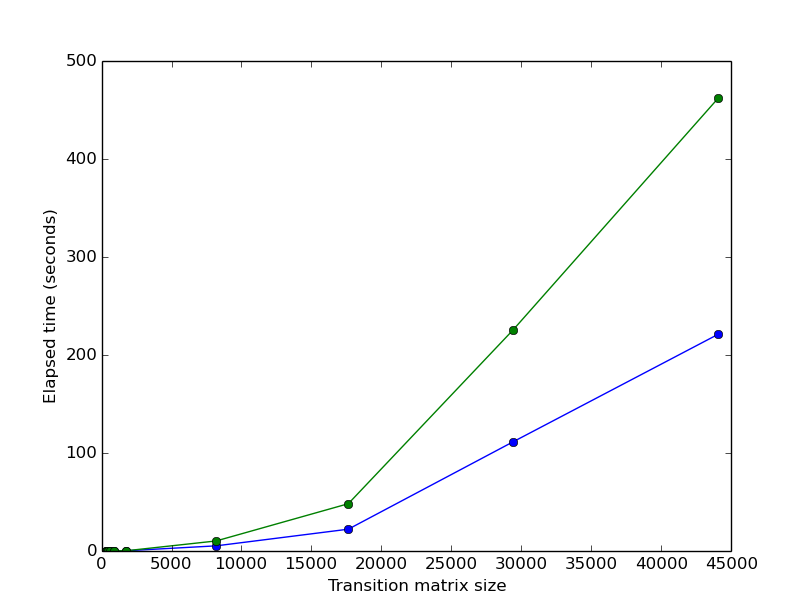
\includegraphics[width=0.6\linewidth]{performance_chart.png}}
  \caption[]{"New" (blue) and "old" (green) algorithm comparison.}
  \label{performancechart}
\end{figure}


The benefits of the new algorithm can be clearly seen also from Figure \ref{performancechart}: as the transition matrix size increases, the difference in terms of elapsed time for its creation grows constantly. The approach developed in this thesis takes about 4 minutes less than the old algorithm with a matrix size of 44080. This test was performed on a server with 64GB of RAM, since the matrix need to fit in memory.